% \title{Apunte de Matemáticas Discretas CC3101:\\ 
% Colorabilidad de Grafos  Clase 21}
% % \title{Ejercicios Lógica e Inducción}
% \author{Andrés Abeliuk}
% \date{}
% \maketitle



\section{Colorabilidad de grafos}

En muchos problemas del mundo real, como la asignación de frecuencias a antenas, la programación de horarios escolares o la resolución de sudokus, surge la necesidad de distinguir elementos conectados entre sí mediante "colores". Esta idea intuitiva está en el corazón de la teoría de coloración de grafos.

El objetivo es sencillo de enunciar: queremos asignar colores a los vértices de un grafo de forma que vértices adyacentes (es decir, conectados por una arista) no compartan el mismo color. Pero como veremos, este problema encierra una profunda riqueza matemática y computacional.

\begin{definitionblock}{Coloración de un grafo}
Una \textbf{coloración} de un grafo simple \( G = (V,E) \) es una asignación de colores a los vértices de \( G \) tal que ningún par de vértices adyacentes recibe el mismo color.
\end{definitionblock}

\bigskip


Es evidente que podemos colorear cualquier grafo simple con \( n \) vértices utilizando \( n \) colores diferentes, asignando un color distinto a cada vértice. No obstante, en la mayoría de los casos, esta cantidad resulta excesiva: muchos grafos permiten una coloración válida con un número significativamente menor de colores.


\noindent A continuación se muestran dos ejemplos de coloración:

\begin{exampleblock}{Ejemplos de coloraciones}
\begin{center}
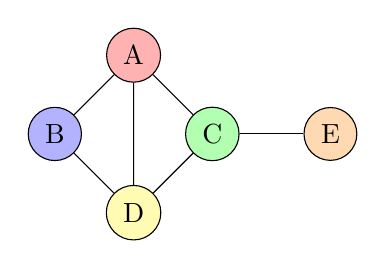
\begin{tikzpicture}[every node/.style={circle, draw, minimum size=5mm}, scale=1]
  \node[fill=red!30] (a) at (0,1) {A};
  \node[fill=blue!30] (b) at (-1,0) {B};
  \node[fill=green!30] (c) at (1,0) {C};
  \node[fill=yellow!30] (d) at (0,-1) {D};
  \node[fill=orange!30] (e) at (2.5,0) {E};
  \draw (a) -- (b) -- (d) -- (c) -- (a) -- (d);
  \draw (c) -- (e);
\end{tikzpicture}
\hspace{1cm}
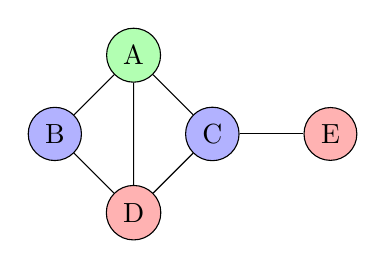
\begin{tikzpicture}[every node/.style={circle, draw, minimum size=5mm}, scale=1]
  \node[fill=green!30] (a) at (0,1) {A};
  \node[fill=blue!30] (b) at (-1,0) {B};
  \node[fill=blue!30] (c) at (1,0) {C};
  \node[fill=red!30] (d) at (0,-1) {D};
  \node[fill=red!30] (e) at (2.5,0) {E};
  \draw (a) -- (b) -- (d) -- (c) -- (a) -- (d);
  \draw (c) -- (e);
\end{tikzpicture}
\end{center}
\end{exampleblock}

En el primer caso se utilizan cinco colores distintos; en el segundo, solo tres. Esto nos lleva a una noción central en teoría de grafos: el \textbf{número cromático}.

\subsection{Número cromático}

\begin{definitionblock}{Número cromático}
El \textbf{número cromático} de un grafo \( G \), denotado \( \chi(G) \), es el menor número de colores necesario para colorear \( G \) de modo que vértices adyacentes tengan colores distintos.
\end{definitionblock}

\bigskip

El número cromático permite clasificar grafos según su complejidad estructural. Por ejemplo:

\begin{itemize}
  \item Un grafo sin aristas tiene número cromático \( \chi = 1 \).
  \item Un grafo bipartito tiene \( \chi = 2 \).
  \item Un ciclo impar tiene \( \chi = 3 \).
  \item Un grafo completo \( K_n \) tiene \( \chi = n \).
\end{itemize}

\begin{exampleblock}{Ejemplos de número cromático}
\begin{center}
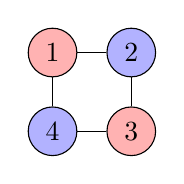
\begin{tikzpicture}[every node/.style={circle, draw, minimum size=5mm}, scale=1]
  \node[fill=red!30] (a) at (0,1) {1};
  \node[fill=blue!30] (b) at (1,1) {2};
  \node[fill=red!30] (c) at (1,0) {3};
  \node[fill=blue!30] (d) at (0,0) {4};
  \draw (a) -- (b) -- (c) -- (d) -- (a);
\end{tikzpicture}
\hspace{1cm}
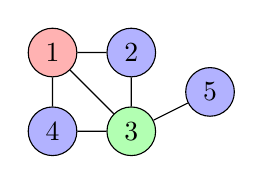
\begin{tikzpicture}[every node/.style={circle, draw, minimum size=5mm}, scale=1]
  \node[fill=red!30] (a) at (0,1) {1};
  \node[fill=blue!30] (b) at (1,1) {2};
  \node[fill=green!30] (c) at (1,0) {3};
  \node[fill=blue!30] (d) at (0,0) {4};
  \node[fill=blue!30] (e) at (2,0.5) {5};
  \draw (a) -- (b) -- (c) -- (d) -- (a) -- (c);
  \draw (c) -- (e);
\end{tikzpicture}
\end{center}
\end{exampleblock}

\bigskip

\noindent En el primer grafo (un ciclo par), el número cromático es \( \chi = 2 \). En el segundo grafo, se requieren tres colores: \( \chi = 3 \).

\bigskip


\subsection{Aplicación: Programación de exámenes}

La Escuela asigna un bloque de tres horas para el examen final de cada ramo. ¿Cuál es la menor cantidad de bloques que puede asignar, de tal manera que los alumnos no tengan tope entre los exámenes de los distintos ramos en los que están inscritos?

\begin{center}
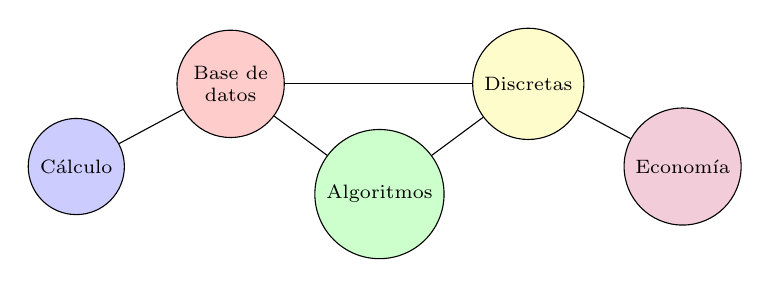
\begin{tikzpicture}[
  every node/.style={
    draw,
    circle,
    minimum size=10mm,
    font=\scriptsize,
    align=center
  },
  scale=0.7
]
  \node[fill=blue!20]   (A) at (0,0)     {Cálculo};
  \node[fill=red!20]    (B) at (2.8,1.5) {Base de\\datos};
  \node[fill=green!20]  (C) at (5.5,-0.5)   {Algoritmos};
  \node[fill=yellow!20] (D) at (8.2,1.5) {Discretas};
  \node[fill=purple!20] (E) at (11,0)    {Economía};

  \draw (A) -- (B);
  \draw (B) -- (C);
  \draw (C) -- (D);
  \draw (D) -- (E);
  \draw (B) -- (D);
\end{tikzpicture}
\end{center}

La respuesta está dada por el número cromático del grafo de incompatibilidad, donde los nodos representan los ramos, y dos nodos son adyacentes si y solo si tienen algún alumno en común.

\subsection{Aplicación: Pintando mapas}

¿Cuál es la mínima cantidad de colores que son necesarios para pintar el siguiente mapa si las regiones limítrofes deben tener distinto color?

\begin{center}
  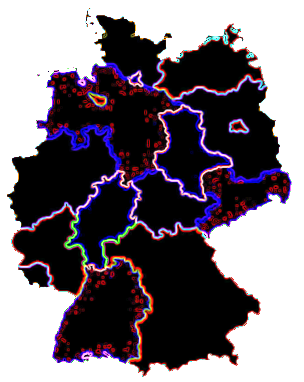
\includegraphics[width=0.2\textwidth]{Figures/MapUnColored.png}
  \hspace{0.5cm}
  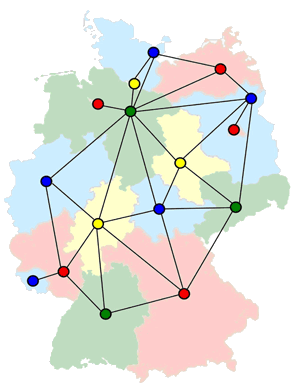
\includegraphics[width=0.2\textwidth]{Figures/MapColored.png}
\end{center}

La respuesta está dada por el número cromático del grafo de la derecha, donde cada vértice representa una región y dos vértices están conectados si las regiones que representan son limítrofes.s.



\section{Grafos planares}

El estudio de coloraciones mínimas está fuertemente ligado a las propiedades geométricas de los grafos, en particular, a su representación en el plano.

\begin{definitionblock}{Grafo planar}
Un grafo es \textbf{planar} si y solo si puede dibujarse en el plano sin que sus aristas se crucen.
\end{definitionblock}

\bigskip

Una representación planar de un grafo divide al plano en \textbf{regiones}, que son las zonas delimitadas por las aristas del grafo cuando este se dibuja en el plano sin cruces. Entre estas regiones siempre se encuentra una región no acotada o exterior, que rodea completamente al dibujo.

Cada vez que una arista o conjunto de aristas encierran una parte del plano sin cruzarse entre sí, forman una región distinta. El número de regiones en una representación planar depende de cómo se conecta el grafo y cuántas aristas y vértices contiene, pero no de cómo se dibuje, siempre que sea una representación planar válida.

Estas regiones son clave en el estudio topológico de grafos, ya que permiten aplicar la fórmula de Euler. También son útiles en aplicaciones como mapas o circuitos, donde evitar cruces mejora la claridad y funcionalidad del diseño.



\begin{exampleblock}{Ejemplo}
La siguiente representación planar divide el plano en 6 regiones:
\begin{center}
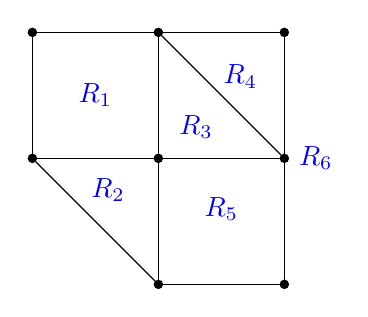
\begin{tikzpicture}[scale=0.8, every node/.style={circle, draw, fill=black, inner sep=1pt, minimum size=3pt}]
  % Nodes
  \node (A) at (0,0) {};
  \node (B) at (2,0) {};
  \node (C) at (4,0) {};
  \node (D) at (0,2) {};
  \node (E) at (2,2) {};
  \node (F) at (4,2) {};
  \node (G) at (2,-2) {};
  \node (H) at (4,-2) {};

  % Edges
  \draw (A) -- (B) -- (C);
  \draw (D) -- (E) -- (F);
  \draw (A) -- (D);
  \draw (B) -- (E);
  \draw (C) -- (F);
  \draw (B) -- (G);
  \draw (C) -- (H);
  \draw (G) -- (H);
  \draw (A) -- (G);
  \draw (E) -- (C);

  % Region labels
  \node[draw=none, fill=none, text=blue] at (1.,1) {$R_1$};
  \node[draw=none, fill=none, text=blue] at (1.2,-0.5) {$R_2$};
  \node[draw=none, fill=none, text=blue] at (2.6,0.5) {$R_3$};
  \node[draw=none, fill=none, text=blue] at (3.3,1.3) {$R_4$};
  \node[draw=none, fill=none, text=blue] at (3,-0.8) {$R_5$};
  \node[draw=none, fill=none, text=blue] at (4.5,0) {$R_6$};
\end{tikzpicture}
\end{center}
\end{exampleblock}


\subsection{Aplicación: Diseño de circuitos eléctricos}

Una aplicación fundamental de los grafos planares se encuentra en el diseño de circuitos eléctricos y microprocesadores. En estos contextos, los componentes electrónicos y sus conexiones se modelan mediante grafos, donde los vértices representan nodos de conexión y las aristas los conductores o enlaces físicos.

\medskip

Para minimizar costos y evitar interferencias, es crucial que el diseño del circuito sea \textbf{planar}, es decir, que las conexiones puedan trazarse en una sola capa sin que se crucen. Si un grafo no es planar, se requieren capas adicionales o el uso de tecnología más costosa para separar conexiones cruzadas.

\begin{center}
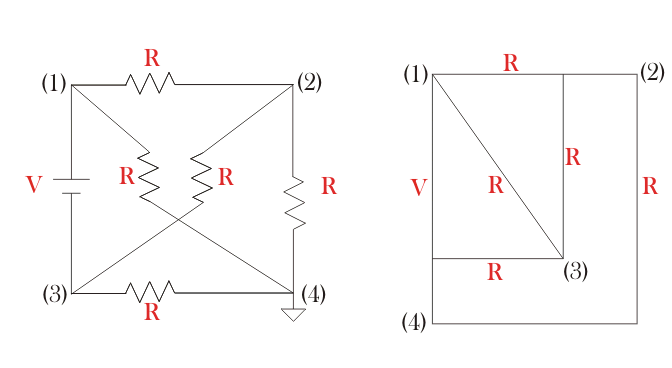
\includegraphics[width=0.5\textwidth]{Figures/planar_circuit.png}
\end{center}

Este problema motiva algoritmos para el reconocimiento de grafos planares y su embebido en el plano.



\subsection{Fórmula de Euler}

Leonhard Euler descubrió una relación entre el número de vértices, aristas y regiones en cualquier grafo planar, conexo y sin múltiples aristas ni lazos. Esta relación es conocida como la \textbf{fórmula de Euler}.


\begin{thmblock}{Fórmula de Euler}
Sea \( G = (V,E) \) un grafo simple, conexo y planar. Sea \( r \) el número de regiones en una representación planar de \( G \). Entonces:
\[
r = |E| - |V| + 2
\]

Esta fórmula es válida para cualquier representación planar del grafo, sin importar su disposición geométrica específica.
\end{thmblock}
\begin{proof}
La demostración se realiza por inducción sobre el número de aristas.
Construimos una secuencia de subgrafos planares:
\[
G_1, G_2, \dots, G_{|E|}
\]
donde cada \( G_{j+1} \) se obtiene al agregar una arista de \( G \) a \( G_j \), de forma que se mantenga la conexidad. Como \( G \) es conexo, siempre podemos agregar una arista que se conecte con los vértices ya presentes.

Demostraremos por inducción que todo \( G_j = (V_j, E_j) \) cumple:
\[
r_j = |E_j| - |V_j| + 2
\]
siendo \( r_j \) el número de regiones de su representación planar.

\textbf{Caso base:} \( G_1 \) tiene una sola arista y dos vértices. Como no encierra ninguna región, \( r_1 = 1 \), y:
\[ r_1 = 1 = 1 - 2 + 2 = 1 \checkmark \]

\textbf{Paso inductivo:} Al agregar una nueva arista, se presentan dos casos:
\begin{itemize}
  \item[(1)] Si une dos vértices ya presentes, crea una nueva región: \( r_{j+1} = r_j + 1 \), \( E_{j+1} = E_j + 1 \) y \( V_{j+1} = V_j \).
  $$\therefore \ {r_{j+1} = |E_{j+1}| - |V_{j+1}| + 2}.$$ 
  \item[(2)] Si introduce un nuevo vértice, no crea regiones: \( r_{j+1} = r_j \), \( E_{j+1} = E_j + 1 \) y \( V_{j+1} = V_j + 1 \).
  $$\therefore \ {r_{j+1} = |E_{j+1}| - |V_{j+1}| + 2}.$$
\end{itemize}

En ambos casos se mantiene:
\[
r_{j+1} = |E_{j+1}| - |V_{j+1}| + 2 \quad \checkmark
\]

Por lo tanto, por inducción, la fórmula se cumple para \( G \).
\end{proof}


\begin{exampleblock}{Ejemplo de Fórmula de Euler}
En el grafo del ejemplo anterior:
\begin{itemize}
  \item Número de vértices: \( |V| = 8 \)
  \item Número de aristas: \( |E| = 12 \)
  \item Número de regiones: \( r = 6 \)
\end{itemize}

Verifiquemos la fórmula:
\[ r = |E| - |V| + 2 = 12 - 8 + 2 = 6 \quad \checkmark \]

La fórmula se cumple.
\end{exampleblock}

\subsection{Corolarios de la fórmula de Euler}
El primer corolario que estudiaremos establece una cota superior para el número de arcos de un grafo planar.
\begin{thmblock}{Corolario 1}
Si \( G \) es un grafo simple, conexo y planar con \( |V| \geq 3 \), entonces:
\[
|E| \leq 3|V| - 6
\]
\end{thmblock}

El siguiente corolario establece una condición necesaria de planaridad.
\begin{thmblock}{Corolario 2}
Todo grafo simple, conexo y planar tiene al menos un vértice de grado a lo sumo 5.
\end{thmblock}

\subsection*{Ejercicios propuestos}

\begin{enumerate}
  \item  Demostrar que el grafo completo \( K_5 \) no es planar.

  \item Sea \( G \) un grafo simple y planar con 9 vértices. ¿Cuál es el máximo número posible de aristas que puede tener?
  \item Da un ejemplo de un grafo conexo que cumple \( |E| \leq 3|V| - 6 \) pero no es planar. ¿Es esto posible?
  \item{*}Demuestra que el grafo bipartito completo \( K_{3,3} \) no es planar, utilizando una variante del Corolario 1 para grafos con ciclos de longitud $\geq4$.
%   \begin{proof} Como en toda representación planar, la suma de los grados de las regiones es igual a dos veces el número de aristas:
% \[
% \sum \deg(R_i) = 2|E|
% \]
% Pero si todos los ciclos tienen longitud \( \geq 4 \), entonces cada región está delimitada por al menos 4 aristas, por lo que:
% \[
% 4|F| \leq 2|E| \Rightarrow 2|F| \leq |E|
% \]
% Aplicando la fórmula de Euler \( |V| - |E| + |F| = 2 \), despejamos \( |F| = |E| - |V| + 2 \) y sustituimos:
% \[
% 2(|E| - |V| + 2) \leq |E| \Rightarrow 2|E| - 2|V| + 4 \leq |E| \Rightarrow |E| \leq 2|V| - 4
% \]
% \end{proof}

\end{enumerate}


\section{Teorema de los Cuatro Colores}

Uno de los resultados más sorprendentes y célebres de la teoría de grafos es el llamado \textbf{Teorema de los Cuatro Colores}. Este surge al estudiar la coloración de grafos planares.

La respuesta, aunque simple, tardó más de un siglo en ser formalmente demostrada.

\begin{thmblock}{Teorema de los Cuatro Colores \textit{(Appel \& Haken, 1976)}}
Sea \( G \) un grafo simple, conexo y planar. Entonces:
\[
\chi(G) \leq 4
\]
Es decir, todo grafo planar puede ser coloreado usando a lo sumo cuatro colores.
\end{thmblock}

Este resultado implica que cualquier mapa, por complejo que sea, puede colorearse con cuatro colores de modo que regiones adyacentes no compartan el mismo color.

\subsection*{Breve historia del teorema}

La conjetura fue planteada en 1852 por Francis Guthrie. A pesar de múltiples intentos fallidos de demostración, no fue hasta 1976 que Kenneth Appel y Wolfgang Haken lograron una prueba definitiva, aunque controversial, utilizando asistencia computacional.

\paragraph{La idea de la demostración.}
Appel y Haken demostraron que no puede existir un \textbf{contraejemplo minimal} al teorema. Para ello, redujeron la verificación a 1.936 configuraciones críticas, las cuales fueron examinadas mediante un algoritmo computacional que corrió durante cientos de horas.

La parte teórica de su demostración ocupa más de 500 páginas, con análisis manual de \textit{contra-contra-ejemplos}. Muchos de estos fueron revisados por el propio hijo de Haken.

El método de demostración generó debate en la comunidad matemática por dos razones. Primero, una parte clave de la prueba fue verificada únicamente por computadora, lo que en su momento generaba desconfianza.
Segundo, la porción escrita a mano era demasiado extensa y engorrosa para que alguien la verificara por completo.


\paragraph{Segunda prueba (Robertson et al., 1997)}

En 1997, Robertson, Sanders, Seymour y Thomas publicaron una nueva prueba del Teorema de los Cuatro Colores en la revista \textit{Journal of Combinatorial Theory}. Esta sigue la misma estrategia general de Appel y Haken, pero con importantes mejoras, por ejemplo, el número de configuraciones se redujo a 633.


\paragraph{Estado actual.} Hasta hoy, no se conoce una demostración del teorema que pueda ser completamente verificada sin asistencia computacional. Aun así, el resultado se acepta universalmente como verdadero, y marca un hito en el uso de computadoras para la demostración matemática.


\subsection{Teoremas de coloración débil para grafos planares}

Además del Teorema de los Cuatro Colores, existen versiones más accesibles que se pueden demostrar con técnicas elementales.

\begin{thmblock}{6-coloración}
Sea \( G \) un grafo simple, conexo y planar. Entonces:
\[ \chi(G) \leq 6 \]
\end{thmblock}

\begin{proof} Por inducción en el número de vértices \( n \).

\textbf{Caso base:} Para \( n \leq 6 \), coloreamos cada vértice con un color distinto.

\textbf{Hipótesis inductiva (HI):} Supongamos que todo grafo planar con \( n-1 \) vértices es 6-colorable.

Sea \( G \) un grafo planar con \( n \) vértices. Por el Corolario del Teorema de Euler, existe un vértice \( v \) de grado a lo sumo 5.

Eliminamos \( v \) y sus aristas incidentes. El grafo restante tiene \( n-1 \) vértices y es 6-colorable por HI.

Entonces podemos colorear \( v \) con un color distinto al de sus (a lo sumo) 5 vecinos.
\end{proof}

\begin{thmblock}{5-coloración}
Sea \( G \) un grafo simple, conexo y planar. Entonces:
\[ \chi(G) \leq 5 \]
\end{thmblock}

\begin{proof}
La demostración también se basa en inducción, pero requiere análisis más delicado sobre cómo intercambiar colores entre vecinos de un nodo \( v \) de grado 5.

\textbf{Caso base:} Todo grafo planar con \( n \leq 5 \) es trivialmente 5-colorable.

\textbf{Hipótesis inductiva (HI):} Todo grafo simple, conexo y planar con \( n-1 \) vértices es 5-colorable.

Sea \( G \) un grafo con \( n \) vértices. Por el Corolario del Teorema de Euler, existe un vértice \( v \) de grado a lo sumo 5. Eliminamos \( v \) y sus aristas incidentes. Por HI, el grafo restante se puede colorear con 5 colores.

Si \( v \) tiene menos de 5 vecinos, al menos un color está disponible para colorearlo. El caso crítico ocurre cuando \( v \) tiene exactamente 5 vecinos con 5 colores distintos.

\begin{center}
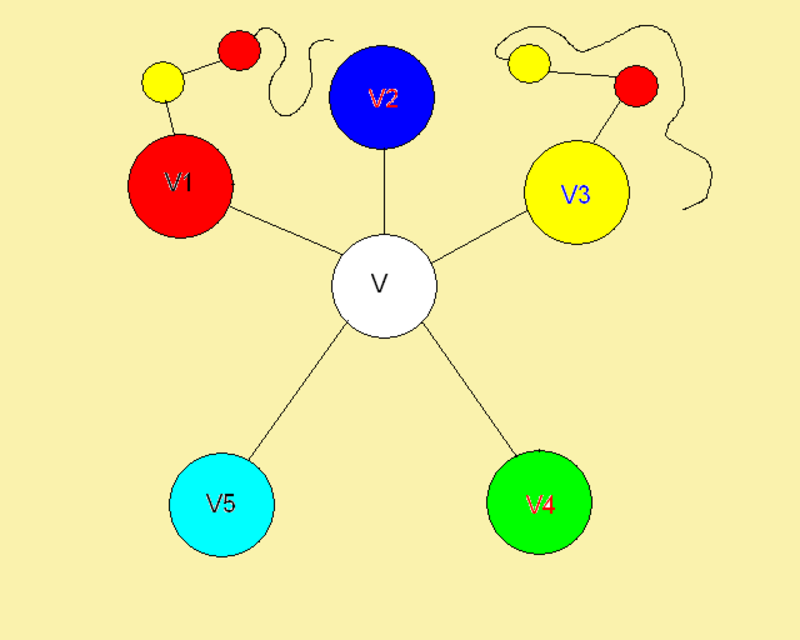
\includegraphics[width=0.3\textwidth]{Figures/fig5color_1}
\end{center}

Sea \( v_1, v_2, v_3, v_4, v_5 \) los vecinos de \( v \), cada uno con un color distinto. Si en el subgrafo inducido por los vecinos, dos vértices con colores \textit{rojo} y \textit{amarillo} (digamos \( v_1 \) y \( v_3 \)) están en componentes diferentes, se puede intercambiar rojo y amarillo en el componente de \( v_1 \), liberando un color para \( v \).

\begin{center}
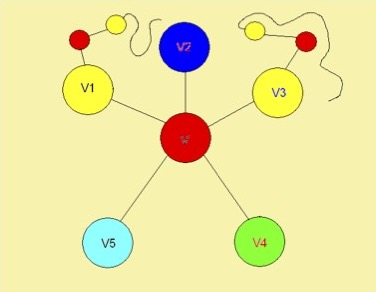
\includegraphics[width=0.3\textwidth]{Figures/fig5color_2}
\end{center}

Si hay un camino entre \( v_1 \) y \( v_3 \), se puede intentar intercambiar otros pares de colores, como \textit{verde} y \textit{azul}:

\begin{center}
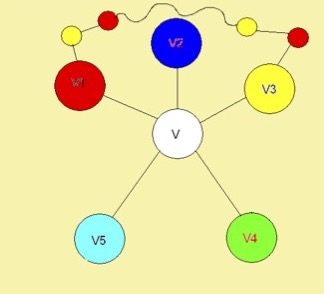
\includegraphics[width=0.3\textwidth]{Figures/fig5color_3}
\end{center}

En el caso extremo en que hay caminos entre \( v_1 \) y \( v_3 \), y también entre \( v_2 \) y \( v_4 \), los caminos deben cruzarse. Esto contradice la planaridad del grafo:

\begin{center}
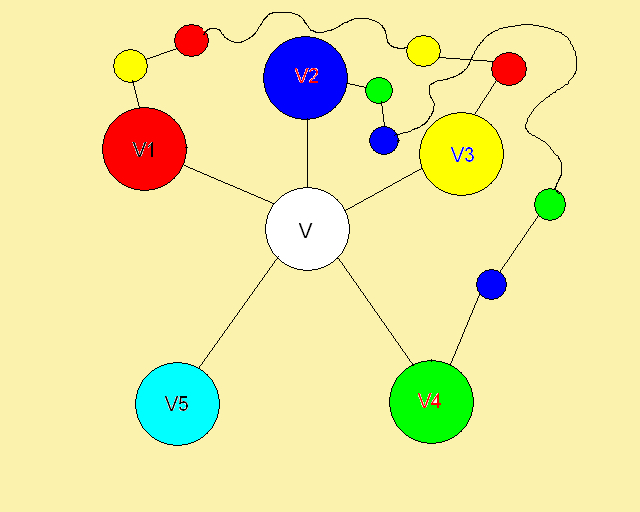
\includegraphics[width=0.35\textwidth]{Figures/fig5color_4}
\end{center}

Por lo tanto, uno de los intercambios de colores es siempre posible, y \( v \) puede ser coloreado con un color distinto a sus vecinos. Esto completa la prueba.
\end{proof}


